\sectionthree{Open and closed; separate chaining}

Now that you know enough about a hash table using an array,
like I said earlier. it's time to talk about another type of hash table.
The above method is called \defone{open addressing}.
Unfortunately, the above is also called \defone{closed hashing}.

Now I'm going to talk about closed addressing which is sometimes called
open hashing and sometimes called separate chaining.
Let me put them together so that you can see everything:
\begin{tightlist}
\li \textsc{Method 1}: Open addressing, closed hashing
\li \textsc{Method 2}: Closed addressing, open hashing, separate chaining.
\end{tightlist}
Obviously computer scientists should come up with better
names.

What I'm going to do now is to allow each bucket
(a row in an array) to have the ability to hold more than one key.
This is easy.
What I'll do is that each row in the array is now replaced by 
containers.
You can choose any container.
But the easiest is to use a linked list, say a singly linked list.

\begin{center}
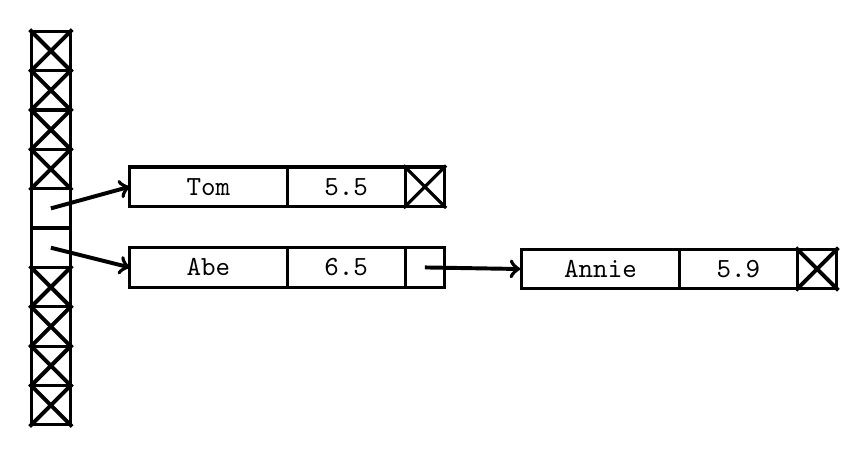
\begin{tikzpicture}
\draw[line width=0.05cm,black] (1.98,0.020000000000000018) to  (2.52,-0.52);
\draw[line width=0.05cm,black] (2.52,0.020000000000000018) to  (1.98,-0.52);
\draw[line width=0.05cm,black] (1.98,-0.48) to  (2.52,-1.02);
\draw[line width=0.05cm,black] (2.52,-0.48) to  (1.98,-1.02);
\draw[line width=0.05cm,black] (1.98,-0.98) to  (2.52,-1.52);
\draw[line width=0.05cm,black] (2.52,-0.98) to  (1.98,-1.52);
\draw[line width=0.05cm,black] (1.98,-1.48) to  (2.52,-2.02);
\draw[line width=0.05cm,black] (2.52,-1.48) to  (1.98,-2.02);

\draw (4.25, -1.975)
  node[draw, line width=0.04cm, , color=black,
       rounded corners=0cm, inner sep=0cm] {

\begin{minipage}[t][0.5cm]{2.0cm}
\mbox{}

\end{minipage}

};\draw (4.25, -1.975) node[color=black] {\texttt{Tom}};
\draw (6.0, -1.975)
  node[draw, line width=0.04cm, , color=black,
       rounded corners=0cm, inner sep=0cm] {

\begin{minipage}[t][0.5cm]{1.5cm}
\mbox{}

\end{minipage}

};\draw (6.0, -1.975) node[color=black] {\texttt{5.5}};
\draw (7.0, -1.975)
  node[draw, line width=0.04cm, , color=black,
       rounded corners=0cm, inner sep=0cm] {

\begin{minipage}[t][0.5cm]{0.5cm}
\mbox{}

\end{minipage}

};\draw[line width=0.05cm,black,->] (2.25,-2.25) to  (3.25,-1.9749999999999999);

\fill[black] (2.25, -2.25) circle (0);
\draw[black] (2.25, -2.25) circle (0.0);\draw[line width=0.04cm,black] (6.73,-1.705) to  (7.27,-2.245);
\draw[line width=0.04cm,black] (7.27,-1.705) to  (6.73,-2.245);

\draw (4.25, -3.0)
  node[draw, line width=0.04cm, , color=black,
       rounded corners=0cm, inner sep=0cm] {

\begin{minipage}[t][0.5cm]{2.0cm}
\mbox{}

\end{minipage}

};\draw (4.25, -3.0) node[color=black] {\texttt{Abe}};
\draw (6.0, -3.0)
  node[draw, line width=0.04cm, , color=black,
       rounded corners=0cm, inner sep=0cm] {

\begin{minipage}[t][0.5cm]{1.5cm}
\mbox{}

\end{minipage}

};\draw (6.0, -3.0) node[color=black] {\texttt{6.5}};
\draw (7.0, -3.0)
  node[draw, line width=0.04cm, , color=black,
       rounded corners=0cm, inner sep=0cm] {

\begin{minipage}[t][0.5cm]{0.5cm}
\mbox{}

\end{minipage}

};\draw[line width=0.05cm,black,->] (2.25,-2.75) to  (3.25,-3.0);

\fill[black] (2.25, -2.75) circle (0);
\draw[black] (2.25, -2.75) circle (0.0);
\draw (9.23, -3.02)
  node[draw, line width=0.04cm, , color=black,
       rounded corners=0cm, inner sep=0cm] {

\begin{minipage}[t][0.5cm]{2.0cm}
\mbox{}

\end{minipage}

};\draw (9.23, -3.02) node[color=black] {\texttt{Annie}};
\draw (10.98, -3.02)
  node[draw, line width=0.04cm, , color=black,
       rounded corners=0cm, inner sep=0cm] {

\begin{minipage}[t][0.5cm]{1.5cm}
\mbox{}

\end{minipage}

};\draw (10.98, -3.02) node[color=black] {\texttt{5.9}};
\draw (11.98, -3.02)
  node[draw, line width=0.04cm, , color=black,
       rounded corners=0cm, inner sep=0cm] {

\begin{minipage}[t][0.5cm]{0.5cm}
\mbox{}

\end{minipage}

};\draw[line width=0.05cm,black] (11.71,-2.75) to  (12.25,-3.29);
\draw[line width=0.05cm,black] (12.25,-2.75) to  (11.71,-3.29);
\draw[line width=0.05cm,black,->] (7.0,-3.0) to  (8.21,-3.0199999999999996);

\fill[black] (7.0, -3.0) circle (0);
\draw[black] (7.0, -3.0) circle (0.0);\draw[line width=0.05cm,black] (1.98,-2.98) to  (2.52,-3.52);
\draw[line width=0.05cm,black] (2.52,-2.98) to  (1.98,-3.52);
\draw[line width=0.05cm,black] (1.98,-3.4800000000000004) to  (2.52,-4.02);
\draw[line width=0.05cm,black] (2.52,-3.4800000000000004) to  (1.98,-4.02);
\draw[line width=0.05cm,black] (1.98,-3.9800000000000004) to  (2.52,-4.52);
\draw[line width=0.05cm,black] (2.52,-3.9800000000000004) to  (1.98,-4.52);
\draw[line width=0.05cm,black] (1.98,-4.48) to  (2.52,-5.02);
\draw[line width=0.05cm,black] (2.52,-4.48) to  (1.98,-5.02);

\draw (2.25, -0.25)
  node[draw, line width=0.04cm, , color=black,
       rounded corners=0cm, inner sep=0cm] {

\begin{minipage}[t][0.5cm]{0.5cm}
\mbox{}

\end{minipage}

};
\draw (2.25, -0.75)
  node[draw, line width=0.04cm, , color=black,
       rounded corners=0cm, inner sep=0cm] {

\begin{minipage}[t][0.5cm]{0.5cm}
\mbox{}

\end{minipage}

};
\draw (2.25, -1.25)
  node[draw, line width=0.04cm, , color=black,
       rounded corners=0cm, inner sep=0cm] {

\begin{minipage}[t][0.5cm]{0.5cm}
\mbox{}

\end{minipage}

};
\draw (2.25, -1.75)
  node[draw, line width=0.04cm, , color=black,
       rounded corners=0cm, inner sep=0cm] {

\begin{minipage}[t][0.5cm]{0.5cm}
\mbox{}

\end{minipage}

};
\draw (2.25, -2.25)
  node[draw, line width=0.04cm, , color=black,
       rounded corners=0cm, inner sep=0cm] {

\begin{minipage}[t][0.5cm]{0.5cm}
\mbox{}

\end{minipage}

};
\draw (2.25, -2.75)
  node[draw, line width=0.04cm, , color=black,
       rounded corners=0cm, inner sep=0cm] {

\begin{minipage}[t][0.5cm]{0.5cm}
\mbox{}

\end{minipage}

};
\draw (2.25, -3.25)
  node[draw, line width=0.04cm, , color=black,
       rounded corners=0cm, inner sep=0cm] {

\begin{minipage}[t][0.5cm]{0.5cm}
\mbox{}

\end{minipage}

};
\draw (2.25, -3.75)
  node[draw, line width=0.04cm, , color=black,
       rounded corners=0cm, inner sep=0cm] {

\begin{minipage}[t][0.5cm]{0.5cm}
\mbox{}

\end{minipage}

};
\draw (2.25, -4.25)
  node[draw, line width=0.04cm, , color=black,
       rounded corners=0cm, inner sep=0cm] {

\begin{minipage}[t][0.5cm]{0.5cm}
\mbox{}

\end{minipage}

};
\draw (2.25, -4.75)
  node[draw, line width=0.04cm, , color=black,
       rounded corners=0cm, inner sep=0cm] {

\begin{minipage}[t][0.5cm]{0.5cm}
\mbox{}

\end{minipage}

};
\end{tikzpicture}

\end{center}


In the above diagram, the array is an array of pointers to singly linked list nodes
or \verb!NULL!.
Of course you can have linked list objects in the array, 
whether the linked list object contain pointers or sentinel nodes.
The linked lists are called chains.

You can think of the above as 10 buckets.
Most of the buckets have no keys.
The bucket at index 4 has one key
and the bucket at index 5 has two keys.

Inserts, deletes, and search are obvious and easy.

Clearly the worse case is measured by the length of the longest singly
linked list in the hash table structure.

When there are many linked lists of long lengths,
of course you can rehash with a largest array.

Besides using linked list, you can of course use balanced trees or even
hash tables at each bucket.



\newpage
